\chapter{Gas Flows and Turbulence}
\label{ch:turbulence}

This chapter covers the physics of turbulence in the cold interstellar medium. This will be something of a whirlwind tour, since turbulence is an entire research discipline unto itself. Our goal is to understand the basic statistical techniques used to describe and model interstellar turbulence, so that we will be prepared to apply them in the context of star formation.

\section{Characteristic Numbers for Fluid Flow}

\subsection{The Conservation Equations}

To understand the origins of turbulence, both in the ISM and more generally, we start by examining the equations of fluid dynamics and the characteristic numbers that they define. Although the ISM is magnetized, we will first start with the simpler case of an unmagnetized fluid. Fluids are governed by a series of conservation laws. The most basic one is conservation of mass:
\begin{equation}
\frac{\partial}{\partial t} \rho = -\nabla \cdot (\rho\mathbf{v}).
\end{equation}
This equation asserts that the change in mass density at a fixed point is equal to minus the divergence of density times velocity at that point. Physically, this is very intuitive: density at a point changes at a rate that is simply equal to the rate at which mass flows into or out of an infinitesimal volume around that point.

We can write a similar equation for conservation of momentum:
\begin{equation}
\frac{\partial}{\partial t}(\rho \mathbf{v}) = -\nabla \cdot(\rho \mathbf{v v}) - \nabla P + \rho \nu \nabla^2 \mathbf{v}.
\end{equation}
Note that the term $\mathbf{vv}$ here is a tensor product. This is perhaps more clear if we write things out in index notation:
\begin{equation}
\frac{\partial}{\partial t}(\rho v_i) = -\frac{\partial}{\partial x_j} (\rho v_i v_j) - \frac{\partial}{\partial x_i} P
+ \rho \nu \frac{\partial}{\partial x_j}\left(\frac{\partial}{\partial x_j} v_i\right)
\end{equation}
The intuitive meaning of this equation can be understood by examining the terms one by one. The term $\rho\mathbf{v}$ is the density of momentum at a point. The term $\nabla \cdot(\rho \mathbf{v v})$ is, in analogy to the equivalent term in the conservation of mass equation, the rate at which momentum is advected into or out of that point by the flow. The term $\nabla P$ is the rate at which pressure forces acting on the fluid change its momentum. Finally, the last term, $\rho \nu \nabla^2 \mathbf{v}$, is the rate at which viscosity redistributes momentum; the quantity $\nu$ is called the kinematic viscosity.

The last term, the viscosity one, requires a bit more discussion. All the other terms in the momentum equation are completely analogous to Newton's second law for single particles. The viscous term, on the other hand, is unique to fluids, and does not have an analog for single particles. It describes the change in fluid momentum due to the diffusion of momentum from adjacent fluid elements. We can understand this intuitively: a fluid is composed of particles moving with random velocities in addition to their overall coherent velocity. If we pick a particular fluid element to follow, we will notice that these random velocities cause some of the particles that make it up diffuse across its boundary to the neighboring element, and some particles from the neighboring element enter. The particles that wander across the boundaries of our fluid element carry momentum with them, and this changes the momentum of the element we're following. The result is that momentum diffuses across the fluid, and this momentum diffusion is called viscosity.

Viscosity is interesting and important because it's the only term in the equation that converts coherent, bulk motion into random, disordered motion. That is to say, the viscosity term is the only one that is dissipative, or that causes the fluid entropy to change. 

\subsection{The Reynolds Number and the Mach Number}

To understand the relative importance of terms in the momentum equation, it is helpful to make order of magnitude estimates of their sizes. Let us consider a system of characteristic size $L$ and characteristic velocity $V$; if we're examining a molecular cloud, we might have $L\sim 10$ pc and $V\sim 5$ km s$^{-1}$. The natural time scale for flows in the system is $L/V$, so we expect time derivative terms to be of order the thing being differentiated divided by $L/V$. Similarly, the natural length scale for spatial derivatives is $L$, so we expect spatial derivative terms to be order the quantity being differentiated divided by $L$. If we apply these scalings to the momentum equation, we expect the various terms to scale as follows:
\begin{equation}
\frac{\rho V^2}{L} \sim \frac{\rho V^2}{L} + \frac{\rho c_s^2}{L} + \rho \nu \frac{V}{L^2},
\end{equation}
where $c_s$ is the gas sound speed, and we have written the pressure as $P = \rho c_s^2$. Canceling the common factors, we get
\begin{equation}
1 \sim 1 + \frac{c_s^2}{V^2} + \frac{\nu}{VL}
\end{equation}

From this exercise, we can derive two dimensionless numbers that are going to control the behavior of the equation. We define the Mach number and the Reynolds number as
\begin{eqnarray}
\mathcal{M} & \sim & \frac{V}{c_s} \\
\mathrm{Re} & \sim & \frac{LV}{\nu}.
\end{eqnarray}
The meanings of these dimensionless numbers are fairly clear from the equations. If $\mathcal{M} \ll 1$, then $c_s^2/V^2 \gg 1$, and this means that the pressure term is important in determining how the fluid evolves. In contrast, if $\mathcal{M} \gg 1$, then the pressure term is unimportant for the behavior of the fluid. In a molecular cloud,
\begin{equation}
c_s  =\sqrt{\frac{k_B T}{\mu m_H}} = 0.18 (T/10\,\mathrm{K})^{1/2},
\end{equation}
where $\mu =2.33$ is the mean mass per particle in a gas composed of molecular hydrogen and helium in the usual cosmic abundance ratio of 1 He per 10 H atoms. Thus $\mathcal{M} V/c_s \sim 20$, and we learn that pressure forces are unimportant.

The Reynolds number is a measure of how important viscous forces are. Viscous forces are significant for $\mathrm{Re} \sim 1$ or less, and are unimportant of $\mathrm{Re} \gg 1$. We can think of the Reynolds number as describing a characteristic length scale $L\sim \nu/V$ in the flow. This is the length scale on which diffusion causes the flow to dissipate energy. Larger scale motions are effectively dissipationless, while smaller scales ones are damped out by viscosity.

To estimate the Reynolds number in the molecular ISM, we must know the viscosity. For an ideal gas, the kinematic viscosity is $\nu=2\overline{u}\lambda$, where $\overline{u}$ is the RMS molecular speed (which is of order $c_s$) and $\lambda$ is the particle mean free-path. The mean free path is of order the inverse of cross-section times density, $\lambda \sim 1/(\sigma n) \sim [(1\mbox{ nm})^2 (100\mbox { cm}^{-3})]^{-1}\sim 10^{12}$ cm. Plugging this in then gives 
$\nu \sim 10^{16}$ cm$^2$ s$^{-1}$ and $\mathrm{Re} \sim 10^9$. Viscous forces are clearly unimportant in molecular clouds.

The extremely large value of the Reynolds number immediately yields a critical conclusion: molecular clouds must be highly turbulent, because flows with $\mathrm{Re}$ of more than $\sim 10^3-10^4$ invariable are. Figure \ref{fig:reynoldsnum_nsf} illustrates this graphically from laboratory experiments.

\begin{figure}
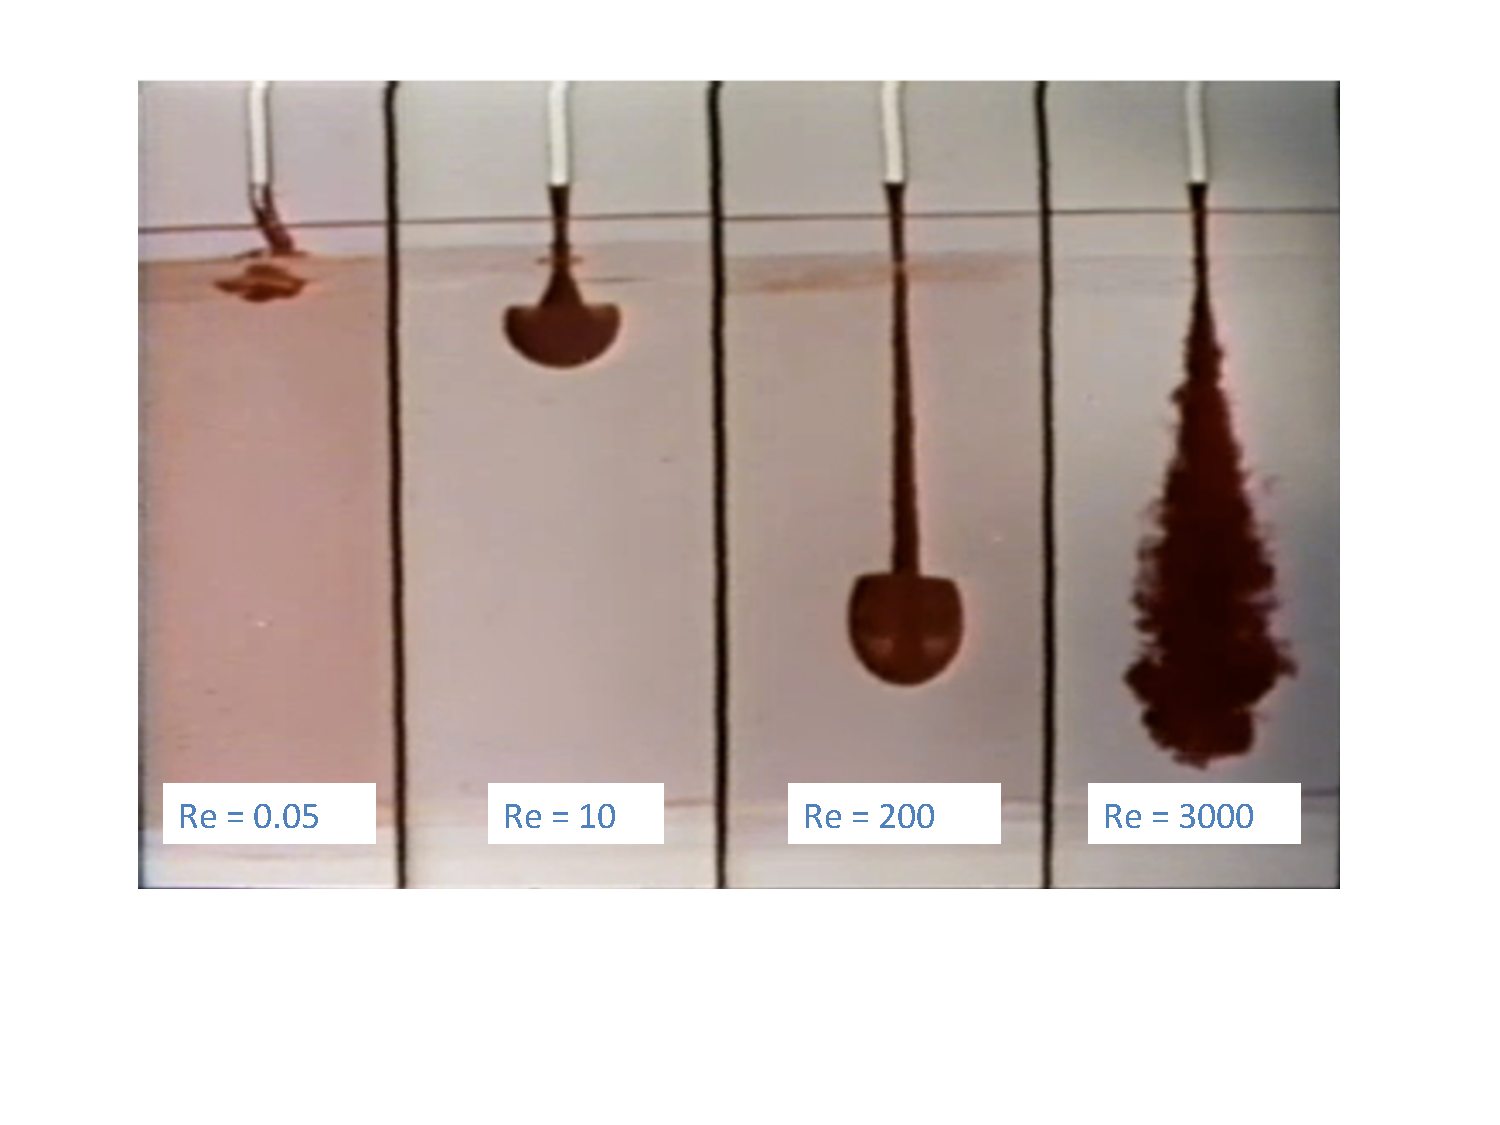
\includegraphics[width=\linewidth]{reynoldsnum_nsf}
\caption[Comparison of Flows at Varying Reynolds Numbers]{
\label{fig:reynoldsnum_nsf}
Flows at varying Reynolds number Re. In each panel, a fluid that has been dyed red is injected from the top into the clear fluid on the bottom. The fluids are a glycerin-water mixture, for which the viscosity can be changed by altering the glycerin to water ratio. By changing the viscosity and the injection speed, it is possible to alter the Reynolds number of the injected flow. The frames show how the flow develops as the Reynolds number is varied. This image is a still from the \href{https://www.youtube.com/playlist?list=PL0EC6527BE871ABA3}{National Committee for Fluid Mechanics Film Series}  \citep{taylor64a}, which, once you get past the distinctly 1960s production values, are a wonderful resource for everything related to fluids.
}
\end{figure}

\section{Modeling Turbulence}

We have remarkably little understanding of how turbulence actually works. However, we have developed some simple models and tools to describe it, and we will next explore those.

\subsection{Velocity Statistics}

One quantity of interest in a turbulent medium is the structure of the velocity field. How does the velocity change from point to point?  In a turbulent medium velocity fluctuates in time and space, and so the best way to proceed is to study those fluctuations statistically. Many statistical tools exist to characterize turbulent motions, and many are used in astrophysics, but we will stick to a few of the simpler ones. We will also make two simplifying assumptions. First we assume that the turbulence is homogenous, in the sense that the turbulent motions do vary only randomly, and not systematically, with position in the fluid. Second, we assume that it is isotropic, so that turbulent motions do not have a preferred directions. Neither of these are likely to be strictly true in a molecular cloud, particularly the second, since large-scale magnetic fields provide a preferred direction, but we will start with these assumptions and relax them later.

Let $\mathbf{v}(\mathbf{x}$ be the velocity at position $\mathbf{x}$. To characterize how this varies with position, we define the autocorrelation function
\begin{equation}
A(\mathbf{r})\equiv \frac{1}{V} \int \mathbf{v}(\mathbf{x})\cdot \mathbf{v}(\mathbf{x}+\mathbf{r}) \, dV \equiv \langle \vecv(\vecx) \cdot \vecv(\vecx+\vecr)\rangle,
\end{equation}
where the angle brackets indicate an average over all positions $\mathbf{x}$. Here, $A(0) = \langle|\vecv|^2\rangle$ is just the RMS velocity in the fluid. If the velocity field is isotropic, then clearly $A(\mathbf{r})$ cannot depend on the direction, and thus must depend only on $r=|\mathbf{r}|$. Thus $A(r)$ tells us how similar or different the velocity is at some scale $r$.

It is often more convenient to think about this in Fourier space than in real space, so rather than the autocorrelation function we often instead think about its Fourier transform. We define the Fourier transform of the velocity field in the usual way, i.e.\
\begin{equation}
\tilde{\vecv}(\veck) = \frac{1}{\sqrt{2\pi}}\int \vecv(\vecx) e^{-i\veck\cdot\vecx} \,d\vecx.
\end{equation}
We then define the power spectrum
\begin{equation}
\Psi(\veck) \equiv | \tilde{\vecv}(\veck)|^2.
\end{equation}

Again, for isotropic turbulence, the power spectrum depends only on the magnitude of the wave number, $k=|\veck|$, not its direction, so it is more common to talk about the power per unit radius in $k$-space,
\begin{equation}
P(k) = 4\pi k^2 \Psi(k).
\end{equation}
This is just the total power integrated over some shell from $k$ to $k+dk$ in $k$-space. Note that Parseval's theorem tells us that
\begin{equation}
\int P(k)\, dk = \int | \tilde{\vecv}(\veck)|^2 \, d^3\veck = \int \vecv(\vecx)^2 \, d^3\vecx,
\end{equation}
i.e.\ the integral of the power spectral density over all wavenumbers is equal to the integral of the square of the velocity over all space, so for a flow with constant density (an incompressible flow) the integral of the power spectrum just tells us how much kinetic energy per unit mass there is in the flow. The Wiener-Khinchin theorem also tells us that $P(\veck)$ is just the Fourier transform of the autocorrelation function,
\begin{equation}
\Psi(\veck) = \frac{1}{(2\pi)^{3/2}} \int A(\vecr) e^{-i\veck\cdot\vecr} \,d\vecr.
\end{equation}

The power spectrum at a wavenumber $k$ then just tells us what fraction of the total power is in motions at that wavenumber, i.e.\ on that characteristic length scale. The power spectrum is another way of looking at the spatial scaling of turbulence. It tells us how much power there is in turbulent motions as a function of wavenumber $k=2\pi/\lambda$. A power spectrum that peaks at low $k$ means that most of the turbulent power is in large-scale motions, since small $k$ corresponds to large $\lambda$. Conversely, a power spectrum that peaks at high $k$ means that most of the power is in small-scale motions.

The power spectrum also tells us about the how the velocity dispersion will vary when it is measured over a region of some characteristic size. Suppose we consider a volume of size $\ell$, and measure the velocity dispersion $\sigma_v(\ell)$ within it. Further suppose that the power spectrum is described by a power law $P(k)\propto k^{-n}$. The total kinetic energy per unit within the region is, up to factors of order unity,
\begin{equation}
\mathrm{KE} \sim \sigma_v(\ell)^2,
\end{equation}
but we can also write the kinetic energy per unit mass in terms of the power spectrum, integrating over those modes that are small enough to fit within the volume under consideration:
\begin{equation}
\mathrm{KE} \sim \int_{2\pi/\ell}^\infty P(k) \, dk \propto \ell^{n-1}
\end{equation}
It therefore follows immediately that
\begin{equation}
\label{eq:vdisp}
\sigma_v = c_s \left(\frac{\ell}{\ell_s}\right)^{(n-1)/2},
\end{equation}
where we have normalized the relationship by defining the sonic scale $\ell_s$ as the size of a region within which the velocity dispersion is equal to the thermal sound speed of the gas.

\subsection{The Kolmogorov Model and Turbulence Cascades}

The closest thing we have to a model of turbulence is in the case of subsonic, hydrodynamic turbulence; the basic theory for that goes back to \citet{kolmogorov41a}.\marginnote{A translation of \citet{kolmogorov41a} (which is in Russian) can be found in \citet{kolmogorov91a}.} Real interstellar clouds are neither subsonic nor hydrodynamic (as opposed to magnetohydrodynamic), but this theory is still useful for understanding how turbulence works.

Kolmogorov's theory of turbulence begins with the realization that turbulence is a phenomenon that occurs when Re is large, so that there is a large range of scales where dissipation is unimportant. It is possible to show by Fourier transforming the Navier-Stokes equation that for incompressible motion transfer of energy can only occur between adjacent wavenumbers. Energy at a length scale $k$ cannot be transferred directly to some scale $k' \ll k$. Instead, it must cascade through intermediate scales between $k$ and $k'$.

This gives a simple picture of how energy dissipates in fluids. Energy is injected into a system on some large scale that is dissipationless, and it cascades down to smaller scales until it reaches a small enough scale for $\mbox{Re}\sim 1$, at which point dissipation becomes significant. In this picture, if the turbulence is in statistical equilibrium, such that is neither getting stronger or weaker, the energy at some scale $k$ should depend only on $k$ and on the rate of injection or dissipation (which are equal) $\psi$.

This allows us to make the following clever dimensional argument. $k$ has units of $1/L$, i.e.\ one over length. The power spectrum has units of energy per unit mass per unit radius in $k$-space. The energy per unit mass is like a velocity squared, so it has units $L^2/T^2$, and this is divided by $k$, so $P(k)$ has units of $L^3/T^2$. The injection / dissipation rate $\psi$ has units of energy per unit mass per unit time, which is a velocity squared divided by a time, or $L^2/T^3$.

Since $P(k)$ is a function only of $k$ and $\psi$, we can write $P(k) = C k^\alpha \psi^\beta$ for some dimensionless constant $C$, then by dimensional analysis we have
\begin{eqnarray}
\frac{L^3}{T^2} & \sim & L^{-\alpha} \left(\frac{L^2}{T^3}\right)^\beta \\
L^3 & \sim & L^{-\alpha+2\beta} \\
T^{-2} & \sim & T^{-3\beta}\\
\beta & = & \frac{2}{3} \\
\alpha & = & 2\beta - 3 = -\frac{5}{3}
\end{eqnarray}

This immediately tell us three critical things. First, the power in the flow varies with energy injection rate to the $2/3$. Second, this power is distributed such that the power at a given wavenumber $k$ varies as $k^{-5/3}$. This means that most of the power is in the largest scale motions, since power diminishes as $k$ increases. Third, if we now take this spectral slope and use it to derive the scale-dependent velocity dispersion from equation (\ref{eq:vdisp}), we find that $\sigma_v \propto \ell^{1/3}$, i.e., velocity dispersion increase with size scale as size to the $1/3$ power. This is an example of what is known in observational astronomy as a linewidth-size relation -- linewidth because the observational diagnostic we use to characterize velocity dispersion is the width of a line. This relationship tells us that larger regions should have larger linewidths, with the linewidth scaling as the 1/3 power of size in the subsonic regime.

The subsonic regime can be tested experimentally on Earth, and Kolmogorov's model provides an excellent fit to observations. Figure \ref{fig:kolmogorov} shows one example.

\begin{figure}
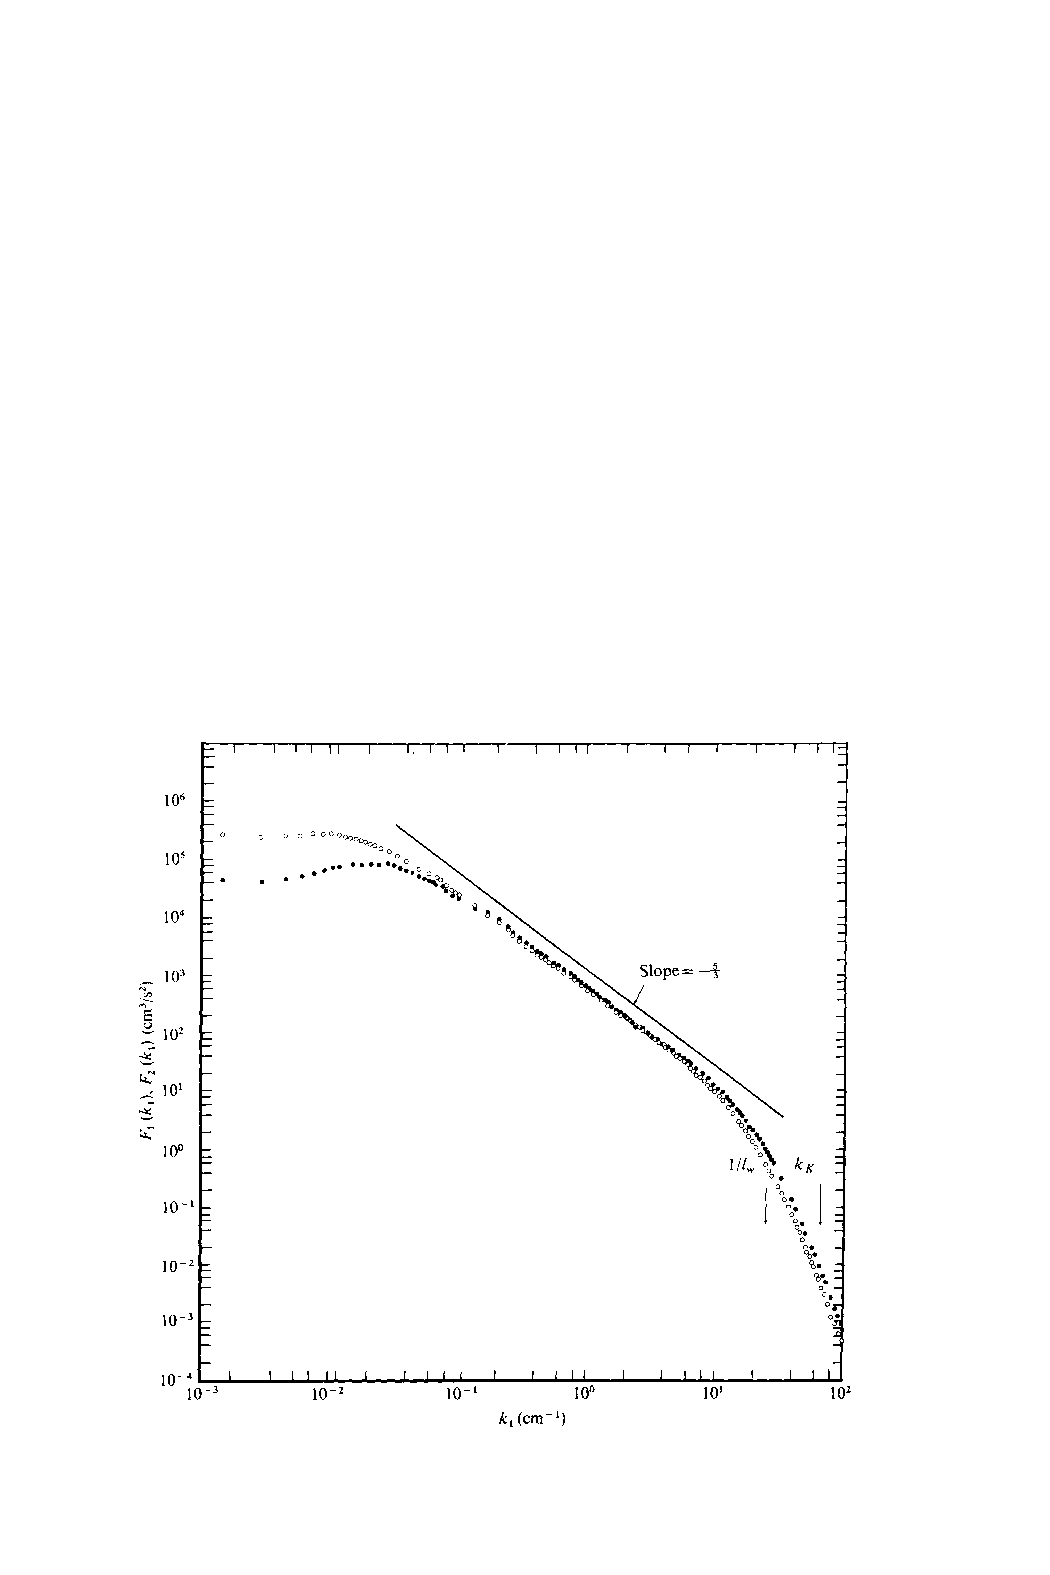
\includegraphics[width=\linewidth]{kolmogorov_champagne78}
\caption[Experimental Power Spectra for Kolmogorov Turbulence]{
\label{fig:kolmogorov}
An experimentally-measured power spectrum for turbulence generated by an air jet \citep{champagne78a}. The $x$ axis is the wavenumber, and the open and filled points show the velocity power spectrum for the velocity components parallel and transverse to the stream, respectively.
}
\end{figure}

\section{Supersonic Turbulence}

\subsection{Velocity Statistics}

We have seen that real interstellar clouds not only have $\mathrm{Re} \gg 1$, they also have $\mathcal{M} \gg 1$, and so the flows within them are supersonic. This means that pressure is unimportant on size scales $L \gg \ell_s$. Since viscosity is also unimportant on large scales (since $\mbox{Re} \gg 1$), this means that gas tends to move ballistically on large scales.

On small scales this will produce very sharp gradients in velocity, since fast-moving volumes of fluid will simply overtake slower ones. Since the viscosity term gets more important on smaller scales, the viscosity term will eventually stop the fluid from moving ballistically. In practice this means the formation of shocks -- regions where the flow velocity changes very rapidly, on a size scale determined by the viscosity. (In real interstellar clouds the relevant viscosity is the magnetic one, as we shall see.)

We expect that the velocity field that results in this case will look like a series of step functions. The power spectrum of a step function is a power law $P(k)\propto k^{-2}$. One can establish this easily from direct calculation. Let's zoom in on the region around a shock, so that the change in velocity on either side of the shock is small. The Fourier transform of $v$ in 1D is
\begin{equation}
\tilde{v}(k) = \frac{1}{\sqrt{2\pi}} \int v(x) e^{-i kx}\, dx
\end{equation}
The periodic function vanishes for all periods in the regions where $v$ is constant. It is non-zero only in the period that includes the shock. The amplitude of $\int v(x) e^{-i kx}\, dx$ during that period is simply proportional to the length of the period, i.e.\ to $1/k$. Thus, $\tilde{v}(k)\propto 1/k$. It then follows that $P(k)\propto k^{-2}$ for a single shock. An isotropic system of overlapping shocks should therefore also look approximately like a power law of similar slope. This gives a velocity dispersion versus size scale $\sigma_v\propto \ell^{1/2}$, and this is exactly what is observed. Figure \ref{fig:polaris} shows an example.

\begin{marginfigure}
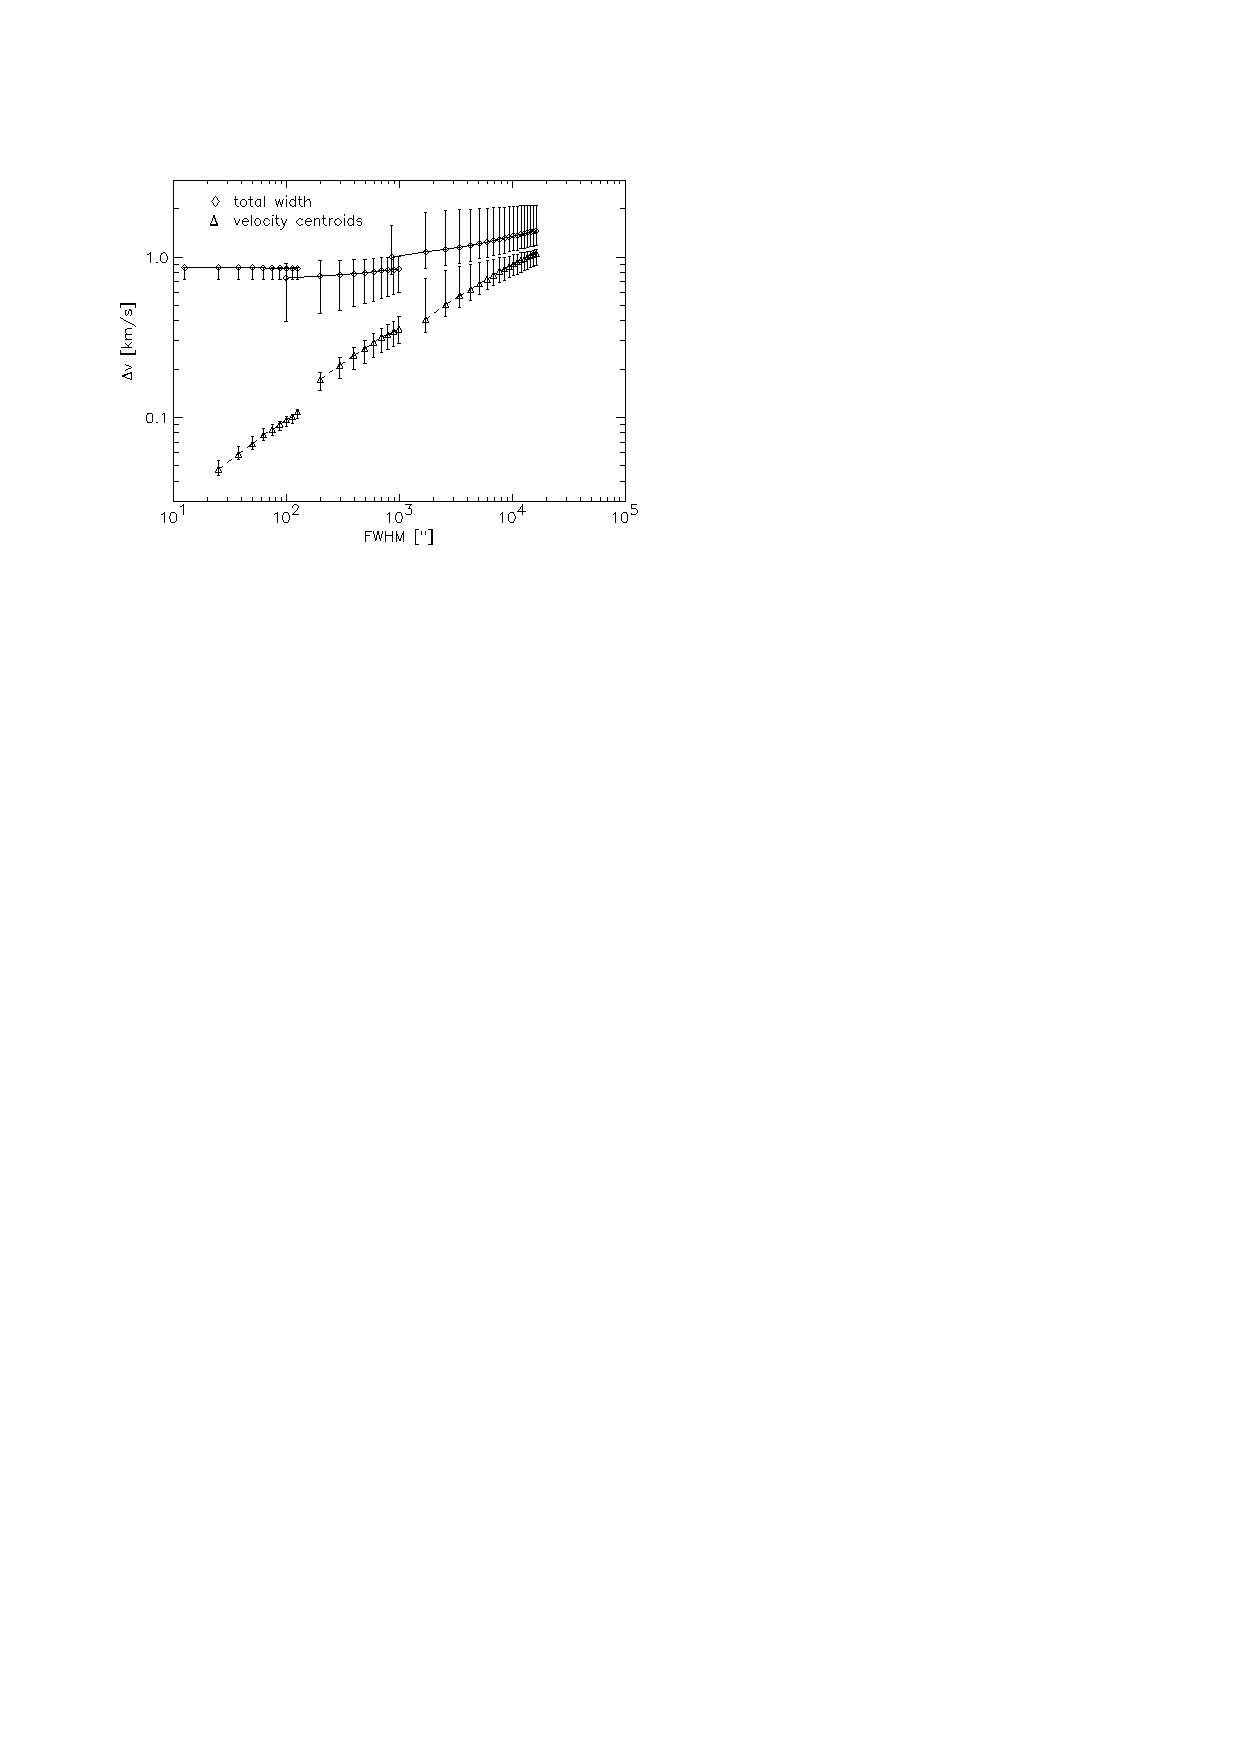
\includegraphics[width=\linewidth]{polaris_ossenkopf02}
\caption[Linewidth versus Size in the Polaris Flare Cloud]{
\label{fig:polaris}
Linewidth versus size in the Polaris Flare Cloud obtained from CO observations \citep{ossenkopf02a}. Diamonds show the total measured velocity width within apertures of the size indicated on the $x$ axis, while triangles show the dispersion obtained by taking the centroid velocity in each pixel and measuring the dispersion of centroids. The three sets of points joined by lines represent measurements from three separate telescopes.
}
\end{marginfigure}

Note that, although the power spectrum is only slightly different than that of subsonic turbulence ($-5/3$ versus about $-2$), there is really an important fundamental difference between the two regimes. Most basically, in Kolmogorov turbulence decay of energy happens via a cascade from large to small scales, until a dissipative scale is reached. In the supersonic case, on the other hand, the decay of energy is via the formation of shocks, and as we have just seen a single shock generates a power spectrum $\propto k^{-2}$, i.e.\ it non-locally couples many scales. Thus, in supersonic turbulence there is no locality in $k$-space. All scales are coupled at shocks.

\subsection{Density Statistics}

In subsonic flows the pressure force is dominant, and so if the gas is isothermal, then the density stays nearly constant -- any density inhomogeneities are ironed out immediately by the strong pressure forces. In supersonic turbulence, on the other hand, the flow is highly compressible. It is therefore of great interest to ask about the statistics of the density field.

Numerical experiments and empirical arguments (but not fully rigorous proofs) indicate that the density field for a supersonically-turbulent, isothermal medium is well-described by a lognormal distribution,
\begin{equation}
\label{eq:denpdf}
p(s) = \frac{1}{\sqrt{2\pi \sigma_s^2}} \exp\left[-\frac{(s-s_0)^2}{2\sigma_s^2}\right],
\end{equation}
where $s=\ln(\rho/\overline{\rho})$ is the log of the density normalized to the mean density $\overline{\rho}$. This distribution describes the probability that the density at a randomly chosen point will be such that $\ln(\rho/\overline{\rho})$ is in the range from $s$ to $s+ds$. The median of the distribution $s_0$ and the dispersion $\sigma_s$ must be related to one another, because we require that
\begin{equation}
\overline{\rho} = \int p(s) \rho \, ds.
\end{equation}
With a bit of algebra, one can show that this equation is satisfied if and only if
\begin{equation}
s_0 = -\sigma_s^2/2.
\end{equation}

Instead of computing the probability that a randomly chosen point in space will have a particular density, we can also compute the probability that a randomly chosen mass element will have a particular density. This more or less amounts to a simple change of variables. Consider some volume of interest $V$, and examine all the material with density such that $\ln(\rho/\overline{\rho})$ is in the range from $s$ to $s+ds$. This material occupies a volume $dV = p(s) V$, and thus must have a mass
\begin{eqnarray}
dM & = & \rho p(s) \, dV \\
& = & \overline{\rho} e^s \cdot \frac{1}{\sqrt{2\pi \sigma_s^2}} \exp\left[-\frac{(s-s_0)^2}{2\sigma_s^2}\right]\,  dV \\
& = & \overline{\rho} \frac{1}{\sqrt{2\pi \sigma_s^2}} \exp\left[-\frac{(s+s_0)^2}{2\sigma_s^2}\right]\,  dV
\end{eqnarray}
\begin{marginfigure}
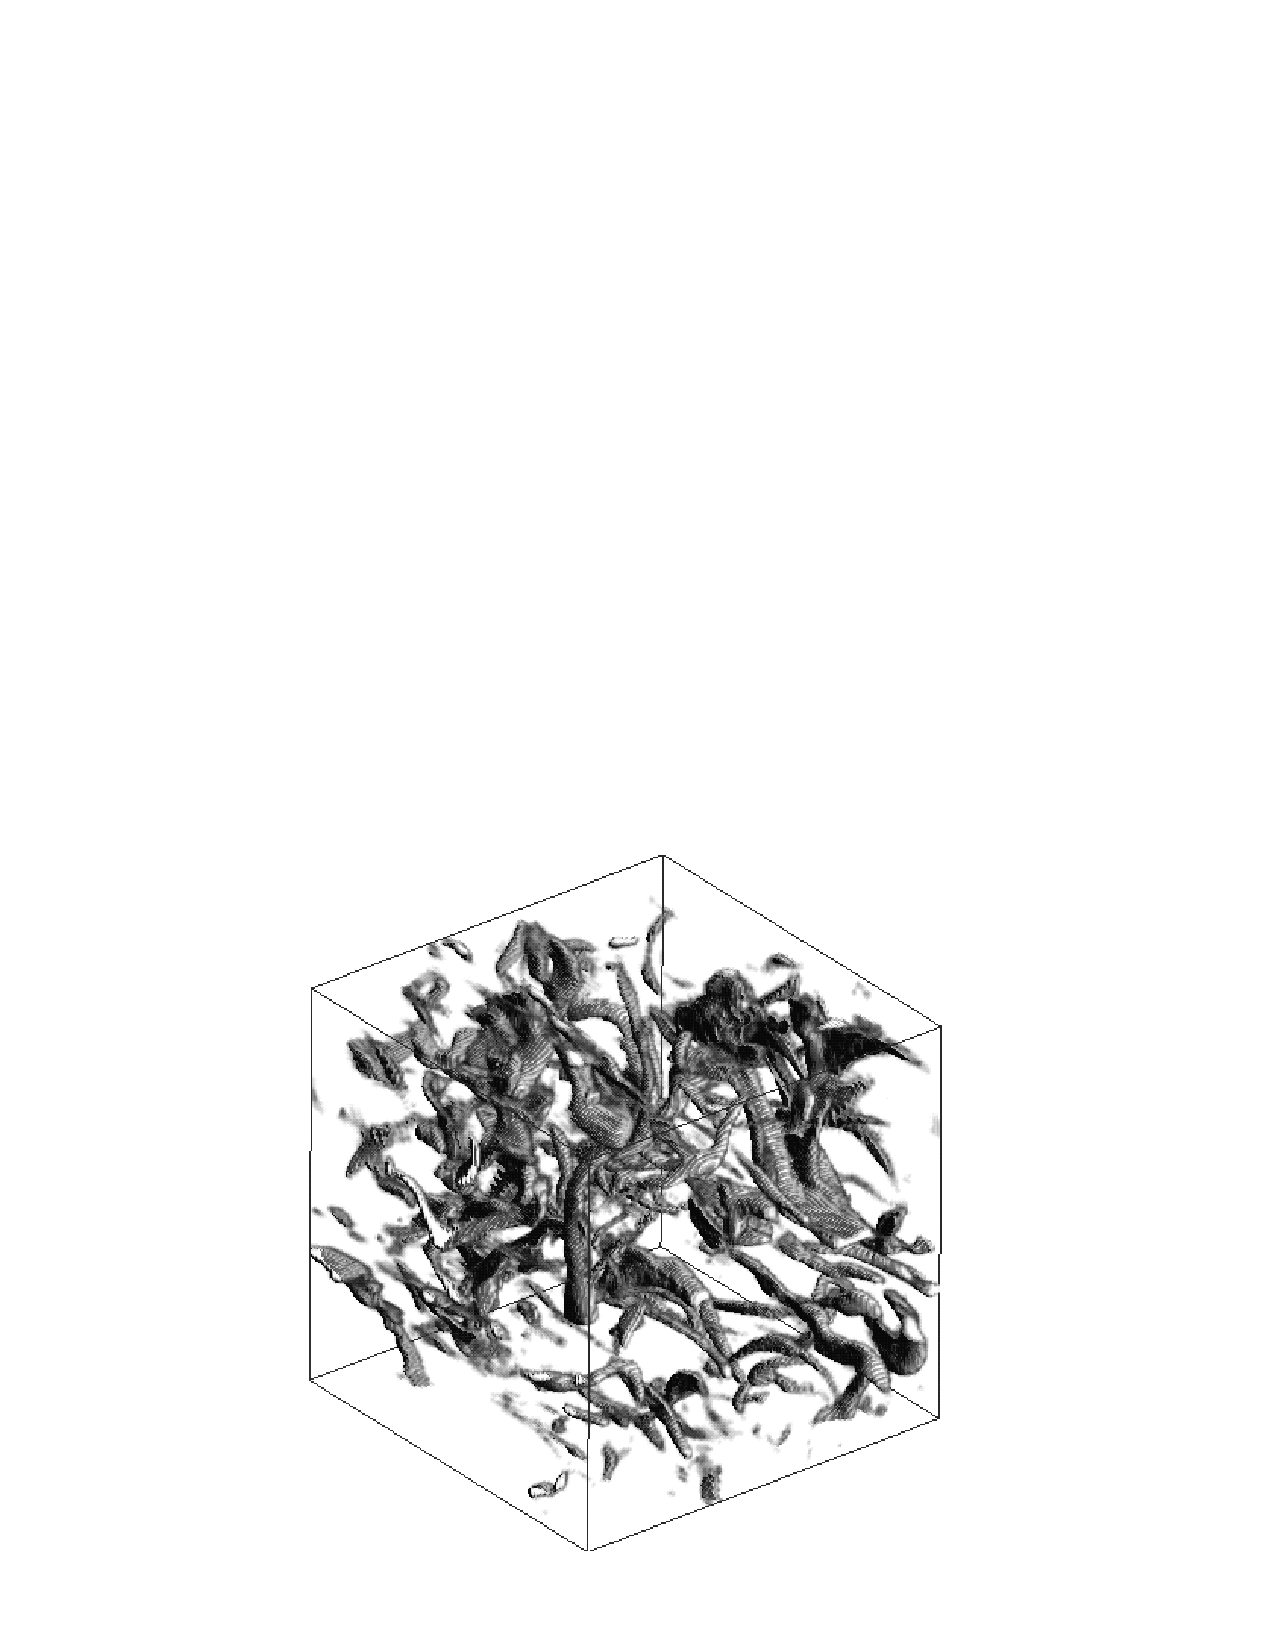
\includegraphics[width=\linewidth]{turbrender_padoan99}
\caption[Volume Rendering of Density Field Supersonic Turbulence]{
\label{fig:turbrender}
Volume rendering of the density field in a simulation of supersonic turbulence \citep{padoan99a}. The surfaces shown are isosurfaces of density.
}
\end{marginfigure}
It immediately follows that the mass PDF is simply
\begin{equation}
p_M(s) = \frac{1}{\sqrt{2\pi \sigma_s^2}} \exp\left[-\frac{(s+s_0)^2}{2\sigma_s^2}\right],
\end{equation}
i.e., exactly the same as the volume PDF but with the peak moved from $-s_0$ to $+s_0$. Physically, the meaning of these shifts is that the typical volume element in a supersonic turbulent field is at a density lower than the mean, because much of the mass is collected into shocks. The typical mass element lives in one of these shocked regions, and thus is at higher-than-average density. Figure \ref{fig:turbrender} shows an example of the density distribution produced in a numerical simulation of supersonic turbulence.

The lognormal functional form is not too surprising, given the central limit theorem. Supersonic turbulence consists of an alternative series of shocks, which cause the density to be multiplied by some factor, and supersonic rarefactions, which cause it to drop by some factor. The result of multiplying a lot of positive density increases by a lot of negative density drops at random tends to produce a normal distribution in the multiplicative factor, and thus a lognormal distribution in the density.

This argument does not, however, tell us about the dispersion of densities, which must be determined empirically from numerical simulations. The general result of these simulations \citep[e.g.,][]{federrath13b} is that
\begin{equation}
\sigma_s^2 \approx \ln \left(1 + b^2 \mathcal{M}^2 \frac{\beta_0}{\beta_0+1}\right),
\end{equation}
where the factor $b$ is a number in the range $1/3-1$ that depends on how compressive versus solenoidal the velocity field is, and $\beta_0$ is the ratio of thermal to magnetic pressure at the mean density and magnetic field strength -- we'll get to the magnetic case next.

In addition to the density PDF, there are higher order statistics describing correlations of the density field from point to point. We will defer a discussion of these until we get to models of the IMF, where they play a major role.

\section{Magnetized Turbulence}

We now make our final generalization, to the case where there is a magnetic field present in the flow and magnetic forces are non-negligible.

\subsection{Observing Magnetic Fields}

Before we begin with the theory, a brief digression into observations: how do we even know that magnetic field are present? A very thorough review can be found in \citet{crutcher12a}, from which this short summary is largely extracted. There are several methods that can be used to measure magnetic fields, but the most direct is the Zeeman effect. The Zeeman effect is a slight shift in energy levels of an atom or molecule in the presence of a magnetic field. Ordinarily the energies of a level depend only the direction of the electron spin relative to its orbital angular momentum vector, not on the direction of the net angular momentum vector. However, in the presence of an external magnetic field, states with different orientations of the net angular momentum vector of the atom have slightly different energies due to the interaction of the electron magnetic moment with the external field. This causes a normally single spectral line produced transitions from that level to split into several separate lines at slightly different frequencies.

For the molecules with which we are concerned, the level is normally split into three sublevels -- one at slightly higher frequency than the unperturbed line, one at slightly lower frequency, and one at the same frequency. The strength of this splitting varies depending on the electronic configuration of the atom or molecule in question. For OH, for example, the splitting is $Z=0.98$ Hz/$\mu$G, where the parameter $Z$ is called the Zeeman sensitivity, and the shift is $\Delta \nu = BZ$, where $B$ is the magnetic field strength. One generally wants to look for molecules where $Z$ is as large as possible, and these are generally molecules or atoms that have an unpaired electron in their outer shell. Examples include atomic hydrogen, OH, CN, CH, CCS, SO, and O$_2$.

\begin{marginfigure}
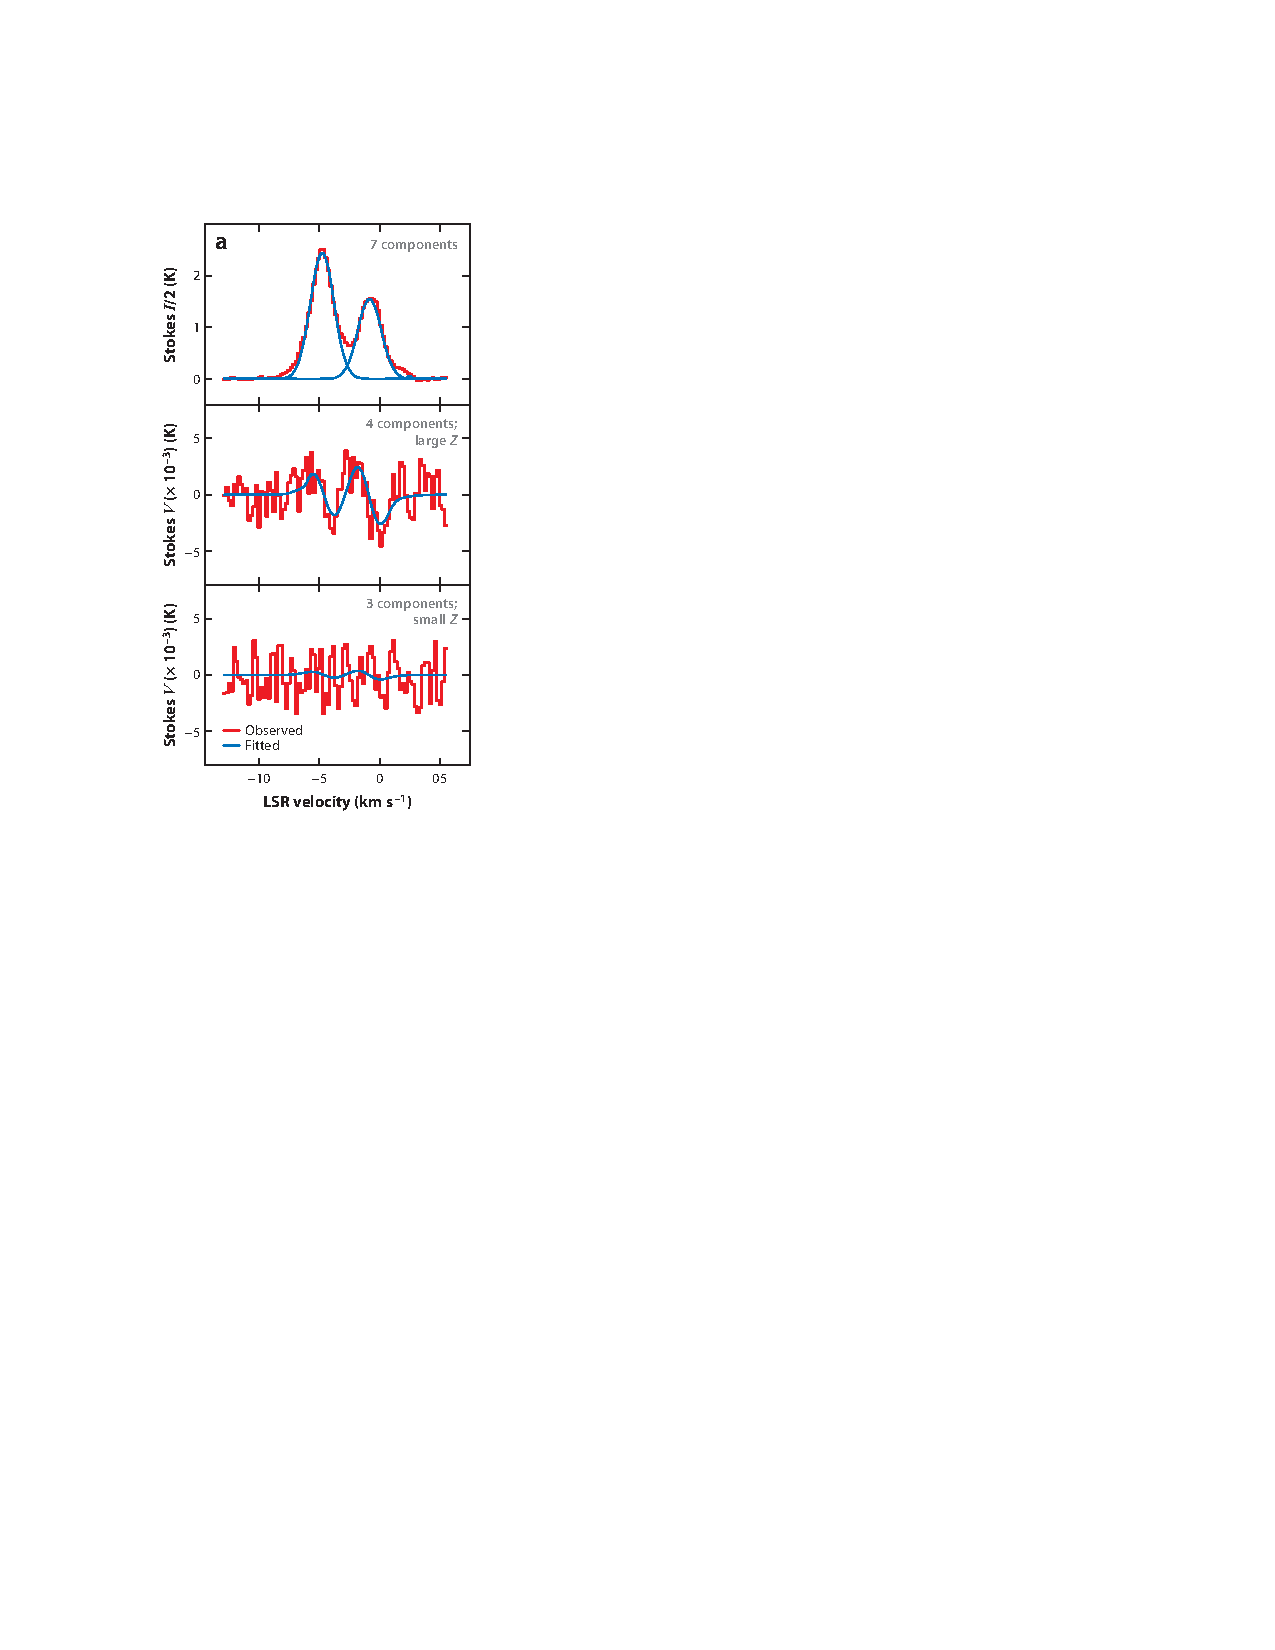
\includegraphics[width=\linewidth]{zeeman_crutcher}
\caption[Sample Zeeman Detection of a Magnetic Field]{
\label{fig:zeeman}
Sample Zeeman detection of an interstellar magnetic field using the CN line in the region DR21(OH) \citep{crutcher12a}. The top panel shows the observed total intensity (Stokes $I$, red lines), which is well-fit by two different velocity components (blue lines). The CN molecule has 7 hyperfine components, of which 4 have a large Zeeman splitting and 3 have a small splitting. The middle panel shows the measured Stokes $V$ (circularly polarized emission) for the sum of the 4 strong splitting components, while the bottom panel shows the corresponding measurement for the 3 weak components. The blue lines show the best fit, with the line of sight magnetic field as the fitting parameter.
}
\end{marginfigure}
The Doppler width of the line is $\sigma_{\nu} = \nu_0 (\sigma_v/c)$, where for the relevant OH transition $\nu_0=1.667$ GHz. If the OH molecule has a velocity dispersion of order $0.1$ km s$^{-1}$, as expected for the lowest observed velocity dispersion even on small scales in molecular clouds, then $(\sigma_v/c)\sim 10^{-6}$, so $\sigma_{\nu} \sim 1$ kHz. This means that, unless the field is considerably larger than $1000$ $\mu$G (1 mG), which it essentially never is, the Zeeman splitting is smaller than the Doppler line width, and we won't see the line split.

However, there is a trick to avoid this problem: radiation from the different Zeeman sublevels has different polarization. If the magnetic field is along the direction of propagation of the radiation, emission from the higher frequency Zeeman sublevel is right circularly polarized, while radiation from the lower frequency level is left circularly polarized. The unperturbed level is unpolarized. Thus although one cannot see the line split if one looks at total intensity (as measured by the Stokes $I$ parameter), one can see that the different polarization components peak at slightly different frequencies, so that the circularly polarized spectrum (as measured by the Stokes $V$ parameter) looks different than the total intensity spectrum. One can deduce the magnetic field strength along the line of sight from the difference between the total and polarized signals. Figure \ref{fig:zeeman} shows a sample detection.

Applying this technique to molecular line emission from molecular clouds indicates that they are threaded by magnetic fields whose strengths range from tens to thousands of $\mu$G, with higher density gas generally showing stronger fields. We can attempt to determine if this is dynamically important by a simple energy argument.

For a low-density envelope of a GMC with $n\sim 100$ cm$^{-3}$ ($\rho \sim 10^{-22}$ g cm$^{-3}$), we might have $v$ of a few km s$^{-1}$, giving a kinetic energy density
\begin{equation}
E_K \sim \rho v^2 \sim 10^{-22}\mbox{ g cm}^{-3} \times (3\times 10^5\mbox{ cm s}^{-1})^2\sim 10^{-11}\mbox{ erg cm}^{-3}.
\end{equation}
The energy density in a magnetic field is
\begin{equation}
E_B = \frac{B^2}{8\pi} \sim \frac{(10\,\mu\mbox{G})^2}{8\pi} \sim 10^{-11} \mbox{ erg cm}^{-3}.
\end{equation}
Thus the magnetic energy density is comparable to the kinetic energy density, and is dynamically significant in the flow.

\subsection{Equations and Characteristic Numbers for Magnetized Turbulence}

To understand how magnetic fields affect the flows in molecular clouds, it is helpful to write down the fundamental evolution equation for the magnetic field in a plasma (this is derived in many places -- my notation and discussion follow Shu's book):
\begin{equation}
\frac{\partial \vecB}{\partial t} + \nabla \times (\vecB \times \vecv) = -\nabla \times (\eta \nabla \times \vecB)
\end{equation}
Here $\vecB$ is the magnetic field, $\vecv$ is the fluid velocity (understood to be the velocity of the ions, which carry all the mass), and $\eta$ is the electrical resistivity. If the resistivity is constant in space, we can use the fact that $\nabla \cdot \vecB=0$ to simplify this slightly to get
\begin{equation}
\frac{\partial \vecB}{\partial t} + \nabla \times (\vecB \times \vecv) = \eta \nabla^2 \vecB.
\end{equation}
The last term here looks very much like the $\nu\nabla^2 \vecv$ term we had in the momentum equation to describe viscosity. That term described diffusion of momentum, while the one in this equation describes diffusion of the magnetic field.

(Note that we're simplifying a bit here -- the real dissipation mechanism in molecular clouds is not simple resistivity, it is something more complex called ambipolar drift, which we'll discuss in more detail later. However, the qualitative point we can make is the same, and the algebra is simpler if we use a simple scalar resistivity.)

We can understand the implications of this equation using dimensional analysis much as we did for the momentum equation. Again, we let $L$ be the characteristic size of the system and $V$ be the characteristic velocity, so $L/V$ is the characteristic timescale. We let $B$ be the characteristic magnetic field strength. Inserting the same scalings as before, the terms vary as
\begin{eqnarray}
\frac{BV}{L} + \frac{BV}{L} & \sim & \eta \frac{B}{L^2} \\
1 & \sim & \frac{\eta}{VL}
\end{eqnarray}
In analogy to the ordinary hydrodynamic Reynolds number, we define the magnetic Reynolds number by
\begin{equation}
\mbox{Rm} = \frac{LV}{\eta}.
\end{equation}
Magnetic diffusion is significant only if $\mathrm{Rm} \sim 1$ or smaller.

What is Rm for a typical molecular cloud? As in the hydrodynamic case, we can take $L$ to be a few tens of pc and $V$ to be a few km s$^{-1}$. The magnetic field $B$ is a few tens of $\mu$G. The electrical resistivity is a microphysical property of the plasma, which, for a weakly ionized plasma, depends on the ionization fraction in the gas and the ion-neutral collision rate. Its typical value for the molecular cloud example we've been using, which we will calculate in a bit, is $\eta\sim 10^{22}-10^{23}$ cm$^2$ s$^{-1}$. Since, as we discussed earlier, $LV\sim 10^{25}$ cm$^2$ s$^{-1}$, this implies that the Rm for molecular clouds is hundreds to thousands.

Again in analogy to hydrodynamics, this means that on large scales magnetic diffusion is unimportant for molecular clouds -- although it is important on smaller scales. The significance of a large value of Rm becomes clear if we write down the induction equation with $\eta=0$ exactly:
\begin{equation}
\frac{\partial \vecB}{\partial t} + \nabla \times (\vecB \times \vecv) = 0.
\end{equation}

To understand what this equation implies, it is useful consider the magnetic flux $\Phi$ threading some fluid element. We define this as
\begin{equation}
\Phi = \int_A  \vecB \cdot \nhat\, dA,
\end{equation}
where we integrate over some area $A$ that defines the fluid element. Using Stokes's theorem, we can alternately write this as
\begin{equation}
\Phi = \oint_C \vecB \cdot d\mathbf{l},
\end{equation}
where $C$ is the curve that bounds $A$. The time derivative of this is then
\begin{eqnarray}
\frac{d\Phi}{dt} & = & \int_A \frac{\partial\vecB}{\partial t}\cdot\nhat\, dA + \oint_C \vecB\cdot \vecv \times d\mathbf{l} \\
& = & \int_A \frac{\partial\vecB}{\partial t}\cdot\nhat\, dA + \oint_C \vecB\times \vecv \cdot d\mathbf{l}
\end{eqnarray}
Here the second term on the right comes from the fact that, if the fluid is moving at velocity $\vecv$, the area swept out by a unit $d\mathbf{l}$ per unit time is $\vecv\times d\mathbf{l}$, so the flux crossing this area is $\vecB\cdot \vecv\times d\mathbf{l}$. Then in the second step we used the fact that $\nabla\cdot \vecB = 0$ to exchange the dot and cross products.

If we now apply Stokes theorem again to the second term, we get
\begin{eqnarray}
\frac{d\Phi}{dt} 
& = & \int_A \frac{\partial\vecB}{\partial t}\cdot\nhat\, dA + \int_A \nabla\times (\vecB\times \vecv) \cdot \nhat\, dA \\
& = & \int_A \left[\frac{\partial\vecB}{\partial t} + \nabla\times (\vecB\times \vecv)\right]\cdot\nhat\,dA\\
& = & 0
\end{eqnarray}
The meaning of this is that, when Rm is large, the magnetic flux through each fluid element is conserved. This is called flux-freezing, since we can envision it geometrically as saying that magnetic field lines are frozen into the fluid, and move along with it.

Thus on large scales the magnetic field moves with the fluid. However, on smaller scales the magnetic Reynolds number is $\sim 1$, and the field lines are not tied to the gas. We will calculate this scale in a bit. Before that, however, we want to calculate another important dimensionless number describing the MHD flows in molecular clouds.

The momentum equation including magnetic forces is
\begin{equation}
\frac{\partial}{\partial t}(\rho \mathbf{v}) = -\nabla \cdot(\rho \mathbf{v v}) - \nabla P + \rho \nu \nabla^2 \mathbf{v} + \frac{1}{4\pi} (\nabla\times\vecB)\times \vecB,
\end{equation}
and if we make order of magnitude estimates of the various terms in this, we have
\begin{eqnarray}
\frac{\rho V^2}{L} & \sim & -\frac{\rho V^2}{L} + \frac{\rho c_s^2}{L} + \frac{\rho \nu V}{L^2} + \frac{B^2}{L} \\
1 & \sim & 1 + \frac{c_s^2}{V^2} + \frac{\nu}{VL} + \frac{B^2}{\rho V^2}
\end{eqnarray}
The second and third terms on the right hand side we have already defined in terms of $\mathcal{M}= V/c_s$ and $\mathrm{Re} = LV/\nu$. We now define our fourth and final characteristic number,
\begin{equation}
\mathcal{M}_A \equiv \frac{V}{v_A},
\end{equation}
where
\begin{equation}
v_A = \frac{B}{\sqrt{4\pi \rho}}
\end{equation}
is the Alfv\'{e}n speed -- the speed of the wave that, in magnetohydrodynamics, plays a role somewhat analogous to the sound wave in hydrodynamics. In flows with $\mathcal{M}_A \gg 1$, the magnetic force term is unimportant, while in those with $\mathcal{M}_A \ll 1$ it is dominant.

Using our characteristic numbers $n\sim 100$ cm$^{-3}$, $B$ of a few tens of $\mu$G, and $V$ of a few km s$^{-1}$, we see that $v_A$ is of order a few km s$^{-1}$, about the same as the velocity. Thus the flows in molecular clouds are highly supersonic ($\mathcal{M}\gg 1$), but only trans-Alfv\'{e}nic ($\mathcal{M}_A \sim 1$), and magnetic forces have a significant influence. Simulations of turbulence with magnetic fields confirm this, as shown in Figure \ref{fig:alfvenmach}.

\begin{figure}
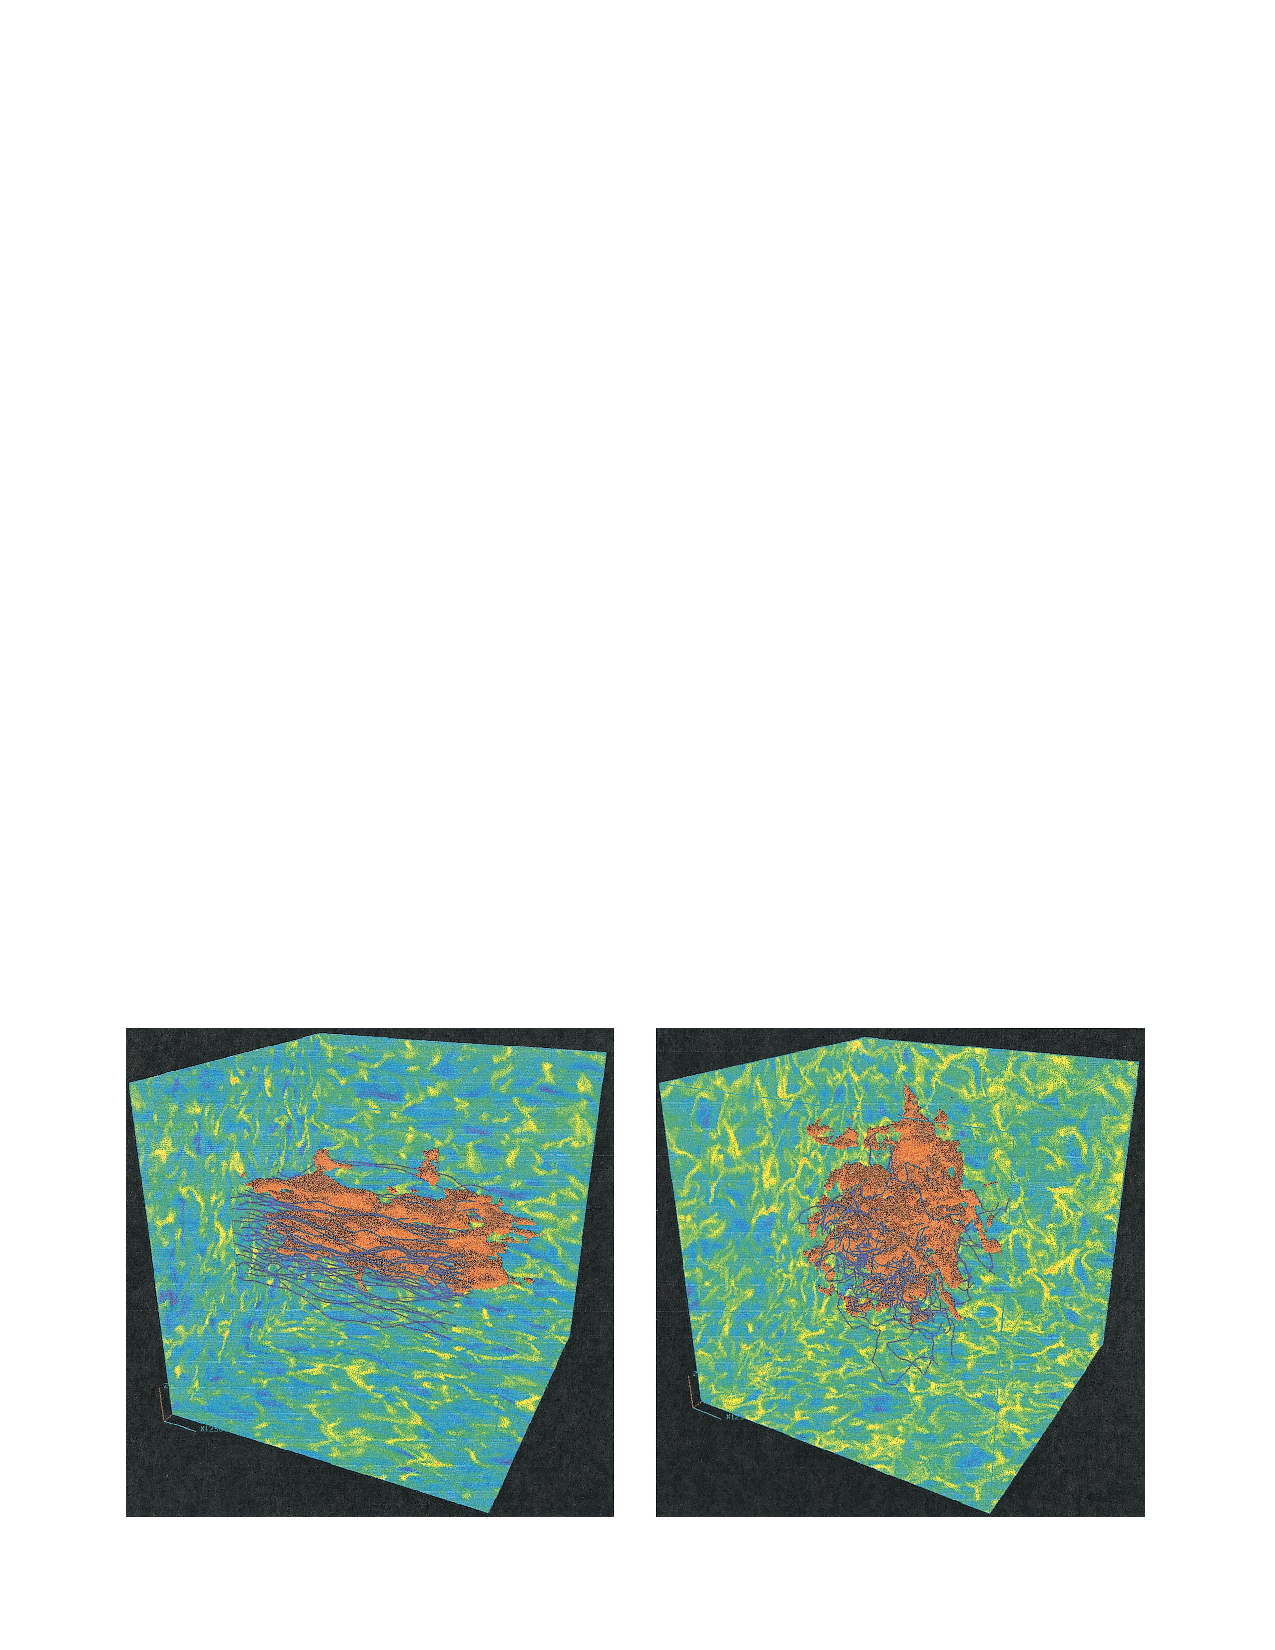
\includegraphics[width=\linewidth]{alfvenmach_stone98}
\caption[Comparison of Simulations of Alfv\'{e}nic and Sub-Alfv\'{e}nic Turbulence]{
\label{fig:alfvenmach}
Simulations of Alfv\'{e}nic (left) and sub-Alfv\'{e}nic (right) turbulence. Colors on the cube surface are slices of the logarithm of density, blue lines are magnetic field lines, and red surfaces are isodensity surfaces for a passive contaminant added to the flow.
}
\end{figure}
